\addtocontents{toc}{\protect\newpage}
\chapter{Concept}
The application should be accessible to all employees of SinnerSchrader. Due to the heterogeneity of the users' computer setups running \textit{Windows}, \textit{macOS} and \textit{Linux}, creating a native application supported by everyone’s system is a rather complicated task. A web application using standard technologies does not only solve this problem, but can also be used from mobile devices such as smartphones and tablets. Furthermore, there is no need to manually install and update the software on the client devices so that it can be assumed that all users use the latest version of the application. This is a positive factor regarding the overall usability of the system and assures bugs and security issues are eliminated the moment a new version of the software is deployed. All those advantages compared to native clients and the fact that SinnerSchrader’s expertise lies in the development of web applications lead to the decision, that such an application would be the appropriate choice.

\section{Person Search}
The central feature of the application is the search function that returns a list of all persons matching the entered set of skills. By default, the results are ordered by a \textit{fitness score} which describes how well a person fits into the set of searched skills.
As the system searches a set of data for a search query entered by the user to return matching items, it falls within the group of \textit{Information Retrieval Systems}.

\subsection{Information Retrieval Systems}
Information Retrieval (IR) systems search a base of data (e.g. documents or websites) for attributes or keywords the user has entered.
Primitive IR systems used search queries combined with boolean operators to specify the searched item, hence they are called \textit{boolean systems}. The commercial solutions examined in \ref{commercial} all use boolean systems.
Modern IR systems ``rank documents by their estimation of the usefulness of a document for a user query'' \cite{IR}, which means they provide more suitable results without the need to enter complex operator based search queries \cite{IR}.

\newpage

\subsection{Search Algorithm}
\label{Search_Algo_Main}
The main feature of the application will be a person search function that uses a ranked IR system to retrieve the most suitable employee for a user's search query.
In the context of this function, all employees are searchable items; their attributes include name, location and their respective skills structured as pairs of skill level and will level. The users will be able to enter the skills they search for and to specify a office location to search at. Minimum levels for skill and will cannot be specified because this would overcomplicate the search query. The IR system will find all employees that offer all skills entered by the user and then rank them so that the most suitable result will be presented first. Due to this ranking approach, the used IR system falls in the category of \textit{Ranked Information Retrieval Systems}.


\subsubsection{Outline}
The basic structure of the IR system's working consists of five steps:
\begin{enumerate}
  \item Create a list of all employees
  \item Filter by Skills\\
    Remove all employees from the list that do not have all skills the user searched for. At this point, only the presence of the skill in the employees' profiles is taken into account; skill/will levels are ignored.
  \item Filter by Location\\
    If the user specified a location to search for, remove all employees from the list that do not match it.
  \item Assign Fitness Scores\\
    Assign a fitness score to all remaining employees. This fitness score takes into account the user's skill/will levels and their specializations.
  \item Sort by fitness score\\
    The results will be sorted by fitness score. The employee with the best fitness score will be shown first in the list of results.
\end{enumerate}

\newpage

\subsubsection{Pseudo-Implementation}
\begin{figure}[!htp]
\begin{lstlisting}[language=Java]
function search(searchItems, searchLocation) {
  var results = getAllEmployees()

  for (Employee e in results) {
    if (!e.skills.containsAll(searchItems)) {
      results.remove(e)
    }
  }

  for (Employee e in results) {
    if (e.location != searchLocation) {
      results.remove(e)
    }
  }

  for (Employee e in results) {
    e.assignFitnessScore()
  }

  results = results.sortByFitnessScore()

  return results
}
\end{lstlisting}
\caption[Pseudocode: Search Algorithm]{Pseudo-Implementation of the search algorithm}
\end{figure}

\newpage

\subsection{Scoring Algorithm}
\label{fitscorealg}
The application will rank all found persons by their fitness into the searched skill set; this fitness will be scored on a scale from zero (worst) to one (best).
The requirements of the algorithm calculating this fitness and its design will be explained in this section.

\subsubsection{Requirements}
According to Spoonamore et al., an algorithm that matches persons to positions that are defined by the skills that are required to fill them has to meet more demands than solely the functional ones. They define the specific requirements such an algorithm assigning naval personnel to positions on a ship as follows:
\blockquote{
\begin{itemize}
  \item Easy to implement and maintain
  \item Fast to execute, so as not to become a computational bottleneck
  \item Takes into account factors: rating, pay grade and NECs\footnote{Navy Enlisted Classifications} and future taxonomies characterizing required knowledge, skills and abilities
\end{itemize}
}
\cite[P. 14]{USN}

\label{customizable}
These qualities include factors very specific to the \textit{US Navy} and thus will have to be evaluated and translated into SinnerSchraders' field of operation, but general requirements such an algorithm has to meet can be deduced: it may not be too complex as employees must be able to understand the system they are rated by, it should take into account different groups of factors and must be easy to adjust in order to keep the system maintainable.

\subsubsection{Factors to Include}
An estimation of a concrete person's fitness into the searched skill set needs not only to take into account the matching of offered and required skills, but also the employees' motivation to apply said skills derived from their preferences and their personal specialization. The latter can be described as the difference between the person's skill/will levels in the searched skill set and their skills that are not part of the search query. In conclusion the factors that will be included in the algorithm are:
\begin{itemize}
  \item Average level of knowledge regarding the searched skills
  \item Average level of will regarding the searched skills
  \item Specialization in the searched skills, derivated from:
  \begin{itemize}
    \item Specialization in knowledge about the searched skills
    \item Preference of the searched skills over others
  \end{itemize}
\end{itemize}


\subsubsection{Proposed Fitness Score Algorithm}
\label{fitnessscore_impl}
As shown in \ref{scale_definition}, the skill and will levels will be described on a four step scale, which will be expressed by natural numbers\footnote{Includes zero as defined by ISO\_80000-2} between zero and three:
\begin{gather*}
  V = \{ x \in \mathbb{N} \ | \  0 \leq x \leq 3\}
\end{gather*}

All existing skills are accumulated in the set $S$. The employee's skills are represented by $E$ which is a subset of $S$. The searched items are
defined as $Q$.

\begin{gather*}
  S = \{Java, Ruby, C++, ...\} \\
  E = \{x \in S \ | \ \textrm{employee has skill x}\} \\
  Q = \{x \in S \ | \ \textrm{user searches for skill x}\}
\end{gather*}

The function $v_s$ assigns a value of skill to any item in $E$; the function $v_w$ assigns the respective level of will to any item in $E$.
\begin{gather*}
  v_s: E \mapsto V \\
  v_w: E \mapsto V
\end{gather*}

The scale values map to terms that describe the person's knowledge or interest:
\begin{center}
\begin{tabular}{c|c|c}
	Value & $v_s$ & $v_w$ \\
	\hline
	0 & novice & uninterested\\
	1 & basic knowledge & indifferent\\
	2 & advanced knowledge & somewhat interested\\
	3 & expert & highly interested\\
\end{tabular}
\end{center}

\newpage

The averages of the employees' skill/will values for the searched skills are defined as $a_s$ and $a_w$.
The variables $s_s$ and $s_w$ describe the employee's specialization in the searched items and are defined as the difference
of the average skill/will level of the searched items and the average level of all other items.
A person with maximal interest and knowledge in all searched items and the lowest ratings in their other items would have the greatest specialization possible and thus get assigned a value of one.

\begin{gather*}
  a_s = \left( \sum_{x \in E \cap Q} v_s(x) \right) \cdot \frac{1}{|E \cap Q|} \\
  a_w = \left( \sum_{x \in E \cap Q} v_w(x) \right) \cdot \frac{1}{|E \cap Q|}
\end{gather*}
\begin{gather*}
  s_s = \frac{max(V) \ + a_s - \left( \left( \sum_{x \in E \setminus Q} v_s(x)\right) \cdot \frac{1}{|E \setminus Q|} \right)}{2 max(V)}\\
  s_w = \frac{max(V) \ + a_w - \left( \left( \sum_{x \in E \setminus Q} v_w(x)\right) \cdot \frac{1}{|E \setminus Q|} \right)}{2 max(V)}
\end{gather*}

The resulting fitness score $f$ is a weighted mean of the introduced factors. The weights $w_{as}$, $w_{aw}$, $w_{ss}$, $w_{sw}$ are positive real numbers and sum up to one.\footnote{Mathematically, this is not necessary, but it results in much more human readable fitness score values between zero and one.}

\begin{gather*}
  f = \frac{w_{as} \cdot a_s}{max(V)} + \frac{w_{aw} \cdot a_w}{ max(V)} + w_{ss} \cdot s_s + w_{sw} \cdot s_w \\
  w_{as} + w_{aw} + w_{ss} + w_{sw} = 1 \\
  w_{as}, w_{aw}, w_{ss}, w_{sw} \in \mathbb{R}^{+} \cup \{0\}
\end{gather*}

\newpage

\subsubsection{Example Calculation}
Let there be three example employees, \textit{Alice}, \textit{Bob} and \textit{Charlie}, having the same three skills each.
(Notation: [skill level]/[will level])
\label{example-fitness}
\newline
\newline
\begin{center}
\begin{tabular}{r|ccc}
  Person  & Java & Ruby & C++ \\
  \hline
  Alice   & 2/1  & 2/2 & 3/3 \\
  Bob     & 2/3  & 0/3 & 0/1 \\
  Charlie & 3/3  & 2/1 & 1/2 \\
\end{tabular}
\end{center}

Applying the algorithm with $w_{as} = w_{aw} = w_{ss} = w_{sw} = 0.25$ to search for the skills \textit{Java} and \textit{Ruby} results in the following values\footnote{Values have been rounded off to two significant digits.}:


\begin{center}
\begin{tabular}{r|cccc|c}
  Person  & $a_s$ & $a_w$ & $s_s$ & $s_w$ & $f$\\
  \hline
  Alice   & 2   & 1.5 & 0.33 & 0.25 & 0.44\\
  Bob     & 1   & 3   & 0.67 & 0.83 & 0.71\\
  Charlie & 2.5 & 2   & 0.75 & 0.5  & 0.69\\
\end{tabular}
\end{center}

Ranking the employees only by the average value of skill regarding the two searched items would result in \textit{Charlie} being preferred to \textit{Alice} and \textit{Alice} being preferred to \textit{Bob}. Sorting them using the proposed fitness score, however, would result in \textit{Bob} being recommended as the best match because his relatively high interest in the searched skills and his specialization in them compensates his low average skill. Interestingly, \textit{Alice} has a better average skill level than \textit{Bob} but nonetheless gets scored the worst due to her obvious specialization in \textit{C++}. In real life usage, the weighting constants $w_{as}$, $w_{aw}$, $w_{ss}$ and $ w_{sw}$ might need to be adjusted.\footnote{The need to adjust the weights should not be considered a flaw since the algorithm has been intendionally designed to be customizable to the users' needs as defined in \ref{customizable}.}

\newpage
\subsection{Example Search}
For this example, let the set of employees be \textit{Alice}, \textit{Bob}, \textit{Charlie}, \textit{Donald}, and \textit{Erika}, and the set of all known skills be \textit{Java}, \textit{Ruby}, and \textit{C++}.
The assignment of skill/will levels and the respective locations are:
\newline
\begin{center}
\begin{tabular}{r|c|ccc}
  Person  & Location & Java & Ruby & C++ \\
  \hline
  Alice   & Hamburg   & 2/1 & 2/2 & 3/3 \\
  Bob     & Hamburg   & 2/3 & 0/3 & 0/1 \\
  Charlie & Hamburg   & 3/3 & 2/1 & 1/2 \\
  Donald  & Hamburg   & 3/3 &  -  & 2/2 \\
  Erika   & Frankfurt & 1/1 & 2/3 & 3/1 \\
\end{tabular}
\end{center}

Let the weights used in the fitness score be $w_{as} = w_{aw} = w_{ss} = w_{sw} = 0.25$.
Applying the algorithm and searching for employees knowing \textit{Java} and \textit{Ruby} in \textit{Hamburg}:\\

\begin{itemize}
  \item Create a list of all employees\\
    $\Rightarrow$ Alice, Bob, Charlie, Donald, Erika
  \item Filter by skills: Donald gets eliminated because he does not have the skill \textit{Ruby}\\
    $\Rightarrow$ Alice, Bob, Charlie, Erika
  \item Filter by location: Erika works in Frankfurt and thus will be excluded\\
    $\Rightarrow$ Alice, Bob, Charlie
  \item Assign fitness scores\footnote{The calculation of the fitness scores can be found in \ref{example-fitness}}\\
    $\Rightarrow$ Alice (0.44), Bob (0.71), Charlie (0.69)
  \item Sort by fitness score\\
    $\Rightarrow$ Bob (0.71), Charlie (0.69), Alice (0.44)
\end{itemize}


\section{Recommender Systems}
Recommender systems ``are information filtering systems that deal with the problem of information overload by filtering vital information fragment out of large amount of [...] information'' \cite{Isinkaye2015261}\label{recommender-definition} and are commonly used to recommend items to the user based on their previous interactions with other items. For example, recommender systems are used to predict products a customer might want to buy based on the ones they already bought in order to present those items more prominently than articles the customer is unlikely to fancy. In this application's context, two recommender systems will come to use in order to enrich the user experience by providing additional skills to search for (see \ref{autocomplete}) and by listing users similar to the currently showed one when the user inspects and employee's profile (see \ref{similar}).

\subsection{Techniques of Content Filtering}
As described by Isinkaye et al., filtering techniques used in recommender systems are divided in three classes: content based, collaborative, and hybrid. Each of these classes relies on a different approach for gaining data by which the information is filtered \cite{Isinkaye2015261}.

\subsubsection{Content Based Filtering}
	The content is filtered by examining its attributes in order to find items that are contentually similar to the one the user is currently or has previously been interacting with.
\subsubsection{Collaborative Filtering}
	Collaborative filtering techniques rely on the assumption that users can be divided into groups of \textit{neighbors} that behave similarly, so that recommendations are deductible from other users' former interactions.
	\begin{itemize}
		\item Model Based Filtering\\
		Model based filtering applies methods of machine learning and data mining to learn a precomputed model which predicts the users' interactions.
		\item Memory Based Filtering\\
		Memory based filtering techniques employ the saved interaction history and generate recommendations based on it. In contrast to model based filtering, memory based filtering does not learn a given model but operates directly on the saved data.
		\begin{itemize}
			\item User Based Filtering\\
			The user's interactions with items are examined in order to find neighbors that share a similar activity history. Once neighbors are found, the system processes their interaction histories in order to find items the user is likely to appreciate getting recommended.
			\item Item Based Filtering\\
			Item based filtering combines all users' interactions and creates a model describing which items are similar to another. This model is then used to recommend items similar to the ones the user has given positive feedback for.
		\end{itemize}
	\end{itemize}
\subsubsection{Hybrid Filtering}
Hybrid filtering combines two or more filtering methods either by aggregating their respective results into a single set of recommendations preferring the items multiple methods recommend, or by bringing content based aspects into the approach of collaborative filtering and vice versa.

\newpage

\subsection{Search Suggestions}
\label{autocomplete}
After entering a skill to look for into the search field, the user will be presented other items they are likely to enter next. Since all searchable objects (all skills) are filtered in order to retrieve objects the user might want to interact with which then will be presented to them proactively, this feature matches the definition of a recommender system given in \ref{recommender-definition}.

\subsubsection{Available Data}
It is not planned that users will have to log in before performing a search, so
there is no user context that can be used to examine a person's former interactions
in order to predict and recommend their next one.\\
As the system is designed to be a web application, a cookie holding a unique identifier could be stored on the client device. The application would then use this ID to aggregate interactions made by the same person. Unfortunately, this method cannot identify a known person using another device because multiple devices will not share the same ID. Furthermore, data collected about a user will be discarded if they delete their devices' cookies or switch browsers.
This approach would also need the application to inform the user that data will be stored on their devices as stated by Article 15(3) of the Telemediengesetz (TMG). The user has to give their approval and must be able to refuse the saving of their data (BDSG, Section 4a).\\
There also are various methods to identify users without the need to store any data on their devices by examining and recognizing their devices' attributes. The collected data can include
factors like language settings, the used browser and its version, and the hardware components of the device. All this data combined can be used to form an almost unique fingerprint suitable to recognize a device \cite{finger}.\\
Another possible method would be to recognize users by examining their very own behavior such as typing patterns or mouse strokes. This approach called \textit{user fingerprinting} does not depend on the user's device and thus can be used to identify people across multiple devices and browsers. On the downside, this method can only differentiate between users typing the same word, it needs a multitude of samples of each user in order to be able to recognize them, and it is very failure-prone \cite{typing}.
Although device and user fingerprinting are not prohibited by law,
the \textit{Opinion 9/2014 on the application of Directive 2002/58/EC to device
fingerprinting} by the EU's \textit{Article 29 data protection working party} states that a user must be informed about the fingerprinting process and be able to deny this.
In the development of this recommender system, it will be assumed that there is no data about unique users, but about their entirety.

\newpage

\subsubsection{Skill Attributes}
The skills are planned to be saved as simple names not enriched with any metainformation, so using content based filtering is not a trivial task. One possible approach would be to use linguistic methods to find similarities in names of skills in order to create clusters of related skills. Unfortunately, most of the skills' names are arbitrarily chosen or acronyms, so that this form of analysis will fail to detect any meaningful attributes.\\
Regarding the concept of the suggestion engine, the assumption is made, that there is no context to the skills and that the only information about any skill is its name.

\subsubsection{Aggregated Search History}
Tracking which skills have been searched together can be implemented easily and creates a fair amount of data to generate potentially useful suggestions. Legally, this is not problematic if the application does neither save personal data about the users (Article 15 Telemediengesetz), nor stores information that could potentially be used to create personal usage profiles that can be matched to specific persons (Article 15(3) Telemediengesetz). Grouping skills that have been searched jointly does not stand in conflict with those regulations and requires no information about distinguishable user, so the application will store the search history for each item.

\subsubsection{Chosen Approach}
Assuming that no user context exist, user based filtering and model based filtering cannot be applied. Due to the lack of metadata about the skills, content based filtering can also be eliminated as a possible approach. Item based filtering, however, does not require any data that is not available, so this approach will be used for the recommender system.

\newpage

\subsubsection{Concept}
The application has access to the list of skills the user already entered into the search field and to a repository of all previous searches. Having this information, the system will use a markov chain to predict the next items that the user is likely to enter and recommend it to them.
Markov chains are stochastic models predicting future states of systems based on the current state. In fact, makrov chains rely on the fact, that the next state of the system is exclusively dependent on the current state, which is called the \textit{markov property} \cite{markprop}. In the context of the skill management application, this is assumed to be true because only two states will be examined: the current state is represented by the set of all items entered in the search field; the future state is the skill set of the current search plus the item the user is going to enter next.
The basic concept is to store all possible states of the system and the respective probability of switching from any state to any other one.
Knowing the current state one can easily deduce the most probable future state. When a state transistion occurs, the outgoing probabilities of the origin states
can be adjusted accordingly in order to factor the transition into the prospective projections.
\begin{figure}[!htp]
    \centering
    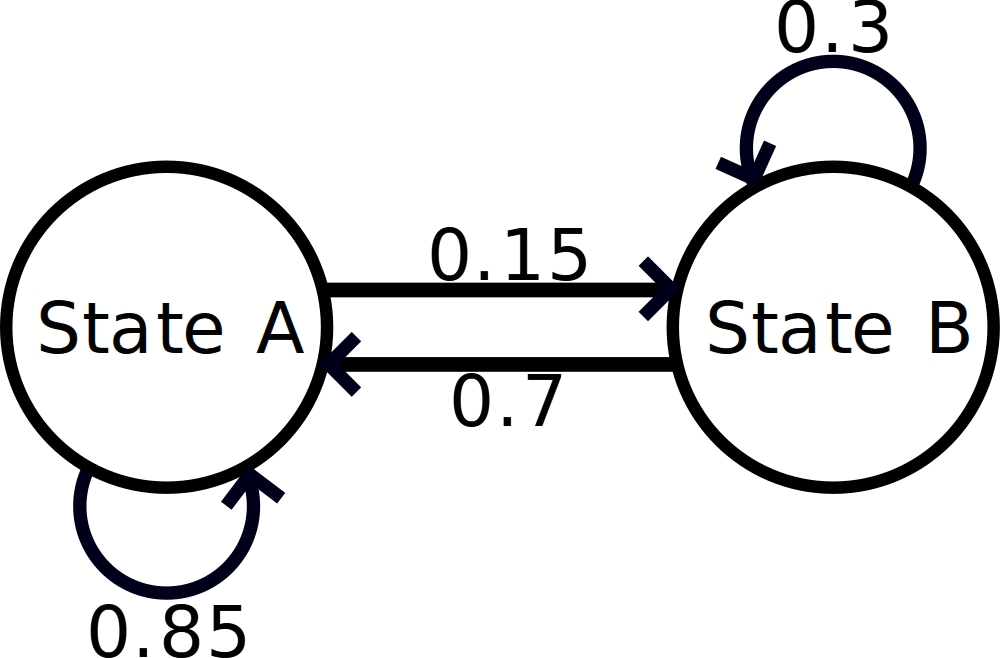
\includegraphics[width=0.33\textwidth]{images/markov-chain.png}
    \caption[Diagram: Markov Chain]{A simple markov chain displayed as a graph. The states are represented as vertices. All possible transitions between states are denoted as edges. The edge weights define the probability of the transition relative to all other outgoing edges of a node.}
    \label{fig:markovchain}
\end{figure}

\newpage

\subsubsection{Data Structure and Algorithm}
An intuitive approach to the implementation of the markov chain generating the search suggestions would be realized by creating one state for every possible combination of skills to search for. State transitions describe the adding of a item to the set of already searched skills, so only transitions from a state to any state that describes the sames skill set plus one more search item are allowed. This approach would result in an exorbitant amount of states (for $n$ skills, there would be $n!$ states) that are overly specific to a single search query, so that recommendations would be based on a small number of previous searches for the exact same combination of skills.
As a tradeoff between keeping the number of states in the markov chain small and generating recommendations specific to the searched skill set, the system will generate predictions for each skill in the search query independently and aggregate these predictions afterwards. For each skill, a list of possible recommendations paired with the total count of searches for both will be stored. The recommendation lists of all skills combined represent the transition matrix. Instead of transition probabilities, the total number of searches is saved in order to simplify the aggreation of multiple suggestions.\\
The recommender system will concatenate the suggestion lists of all items in the current search query and add up the count numbers of skills appearing in multiple suggestion lists. Then, all elements of the combined list that are part of the search query will be removed, the result is a list of suggestions for the whole search query. The items will then be sorted by said search count. The first $n$ elements, where $n$ ist the number of items to recommend, will be returned.\\

\newpage

\subsubsection{Pseudo-Code}
\begin{figure}[!htp]
\begin{lstlisting}[language=Java]
var knownSkills = [
  {
    name: "java",
    searchedWith: [
      {
        name: "php",
        count: 3
      }, {
        name: "ruby",
        count: 2
      }
    ]
  }, {
    name: "php",
    searchedWith: [
      {
        name: "java",
        count: 3
      }, {
        name: "ruby",
        count: 5
      }
    ]
    name: "ruby",
    searchedWith: [
      {
        name: "java",
        count: 2
      }, {
        name: "php",
        count: 5
      }
    ]
  }
]
\end{lstlisting}
\caption[Data Structure: Known Skill]{Pseudo-Implementation of the known skills' data structure}
\end{figure}

\newpage

\begin{figure}[!htp]
\begin{lstlisting}[language=Java]
function suggest(searched, n) {
  var accumulated = {};

  for (s in searched) {
    for (t in knownSkills.getByName(t).searchedWith) {
      if (accumulated.getByName(t) exists) {
        accumulated.getByName(t).count += t.count
      } else {
        accumulated.getByName(t) = t.clone()
      }
    }
  }

  for (t in accumulated) {
    if (searched contains t) {
      remove t from accumulated
    }
  }

  return accumulated.sortByCount().getSubList(0, n)
}

\end{lstlisting}
\caption[Pseudocode: Skill Suggestion Algorithm]{Pseudo-Implementation of the suggestion of a known skill based on a set of already searched items.}
\end{figure}

\newpage

\subsubsection{Example}
Let there be the following transition matrix:

\begin{center}
\begin{tabular}{c | c |c | c | c}
		  & Java & PHP & CSS & COBOL\\
	\hline
	Java  &  -   &  7  &  3  &   1  \\
	\hline
	PHP   &  7   &  -  &  9  &   5  \\
	\hline
	CSS   &  3   &  9  &  -  &   8  \\
	\hline
	COBOL &  1   &  5  &  8  &   -  \\
\end{tabular}
\end{center}

In this example, the query ``Java, PHP'' has already been entered. Based on those elements, one more item shall be recommended to the user ($n = 1$).
\begin{enumerate}
	\item Retrieve suggestion lists for each search item\\
		$\Rightarrow$ PHP (7), CSS (3), COBOL (1), Java (7), CSS (9), COBOL (5)
	\item Aggregate lists (combine counts)\\
		$\Rightarrow$ PHP (7), Java (7), CSS (12), COBOL (6)
	\item Remove suggestions that are part of the search query\\
		$\Rightarrow$ CSS (12), COBOL (6)
	\item Sort by count\\
		$\Rightarrow$ CSS (12), COBOL (6)
	\item Suggest the first $n$ items ($n = 1$)\\
		$\Rightarrow$ CSS
\end{enumerate}

\begin{figure}[!htp]
    \centering
    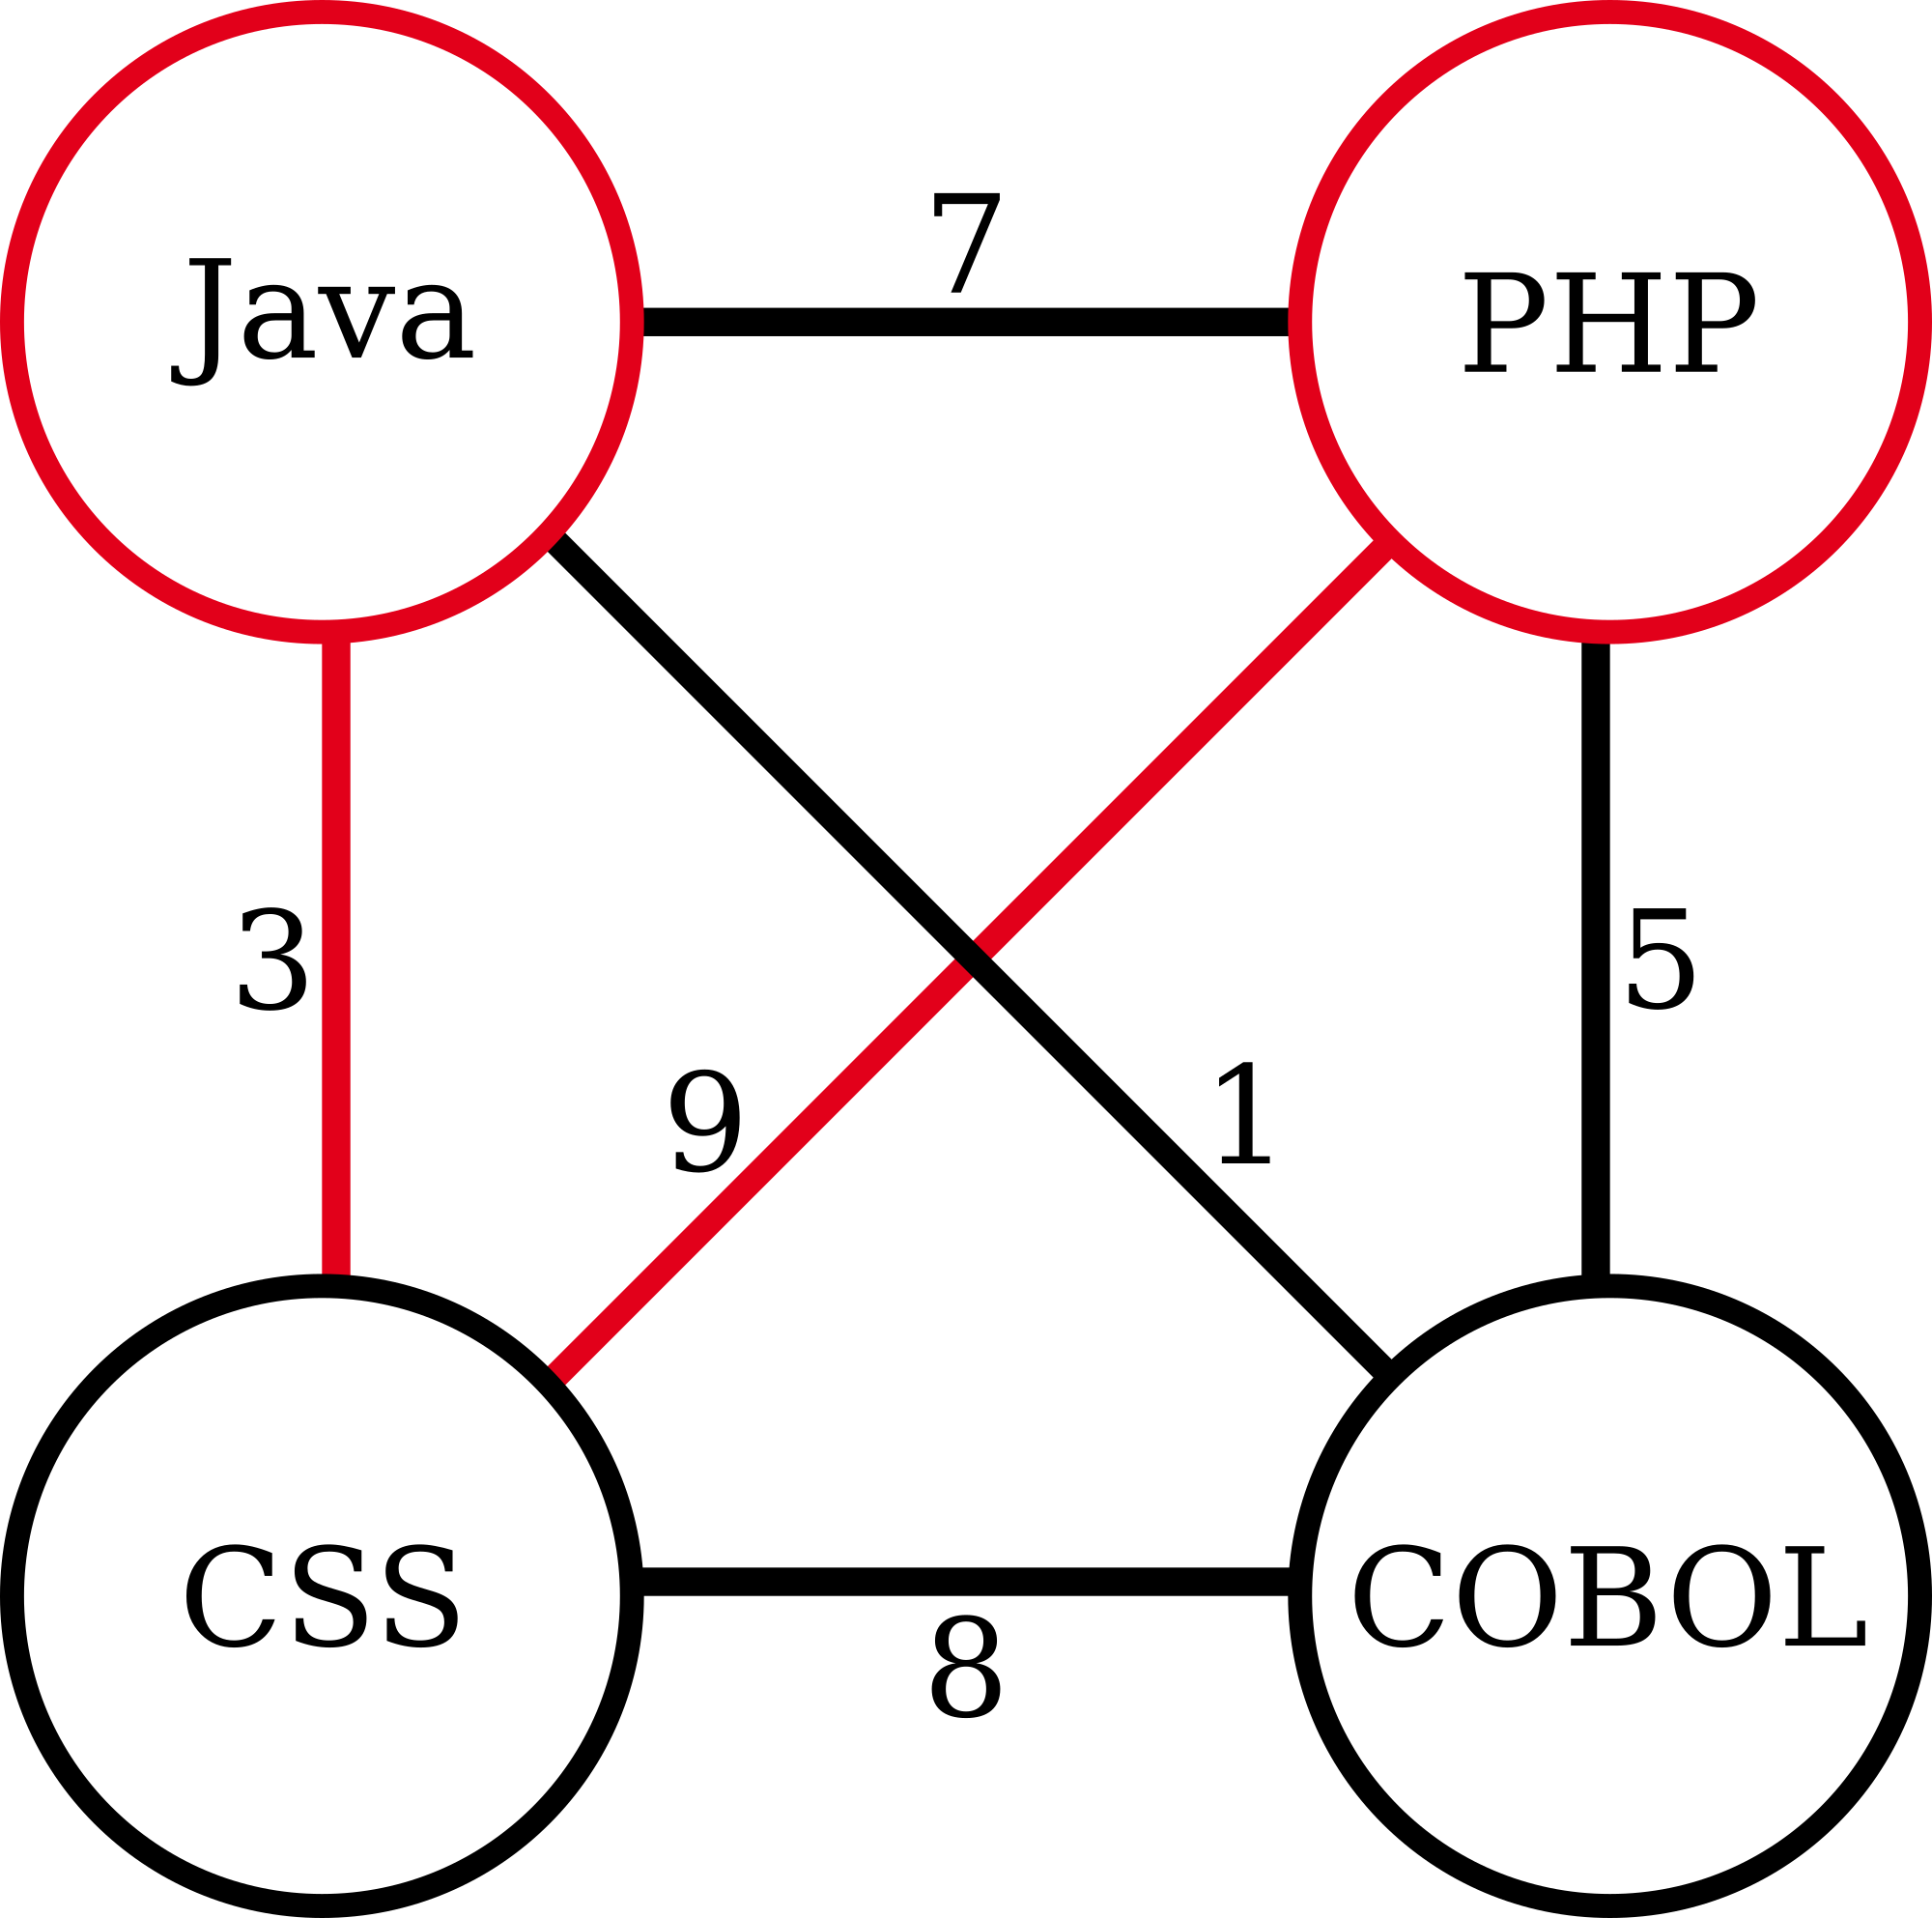
\includegraphics[width=0.33\textwidth]{images/markov_impl.png}
    \caption[Diagram: Search Suggestion Markov Model]{Markov Model used in the example. The two origin states and the transitions that form the end result are highlighted red.}
    \label{fig:wireframe}
\end{figure}

\newpage

\subsection{Recommending Similar Users}
\label{similar}
Additionally to the required features, the backend will provide the possibility to find users that are similar to a reference person.
In the application, this feature will be used to show recommended persons when viewing one specific employee's profile. As this functionality filters the entirety of employees to find the ones that are similar to currently shown profile and then proactively recommends those people to the user, it is another recommender system.
Unlike the recommender system used to provide more skills to search for, this system will use a content-based filtering approach. The employee profiles contain numerous skills that represent a sufficient amount of inherent information about the respective person to compare profiles in order to find similar ones. Other users' interactions with the profiles, however, do not necessarily indicate similarities, so that the interaction history will not be taken into account for this feature. As a consequence, collaborative filtering approaches are not applicable to this problem.
The recommender algorithm will contain three straightforward steps:
\begin{itemize}
	\item Get a list of all users except the reference one
	\item Sort the list by similarity with the reference user
	\item Recommend the first $n$ items in the list ($n$ = number of recommendations to make)
\end{itemize}

\subsubsection{Jaccard Similarity Coefficient}
As shown in \ref{fitnessscore_impl}, users can be described as sets of skills they have, so the task of measuring the similarity between users can be abstracted to estimating the correlation between their skill sets. A popular approach to this problem is using the \textit{Jaccard Similarity Coefficient}, a statistical metric to determine the similitude of two finite sets by dividing the size of their intersection with the size of their union \cite{jaccard}. The resulting value describes how similar the skill sets are and thus represents how similar the respective users are. The results maximum value is one (users are identical); the minimum value is zero (users to not share any skills).\\
Let $S$ be the set of all skills existing in the system. Persons will be described as the sets of skills they have: the employee based on whom the recommendations shall be made will be called $R$ (\textit{reference employee}). The employee whose similarity with $R$ is to be measured will be called $E$.

\begin{gather*}
	S = \{Java, Ruby, C++, ...\} \\
	E = \{x \in S \ | \ \textrm{examined employee has skill x}\} \\
	R = \{x \in S \ | \ \textrm{reference employee has skill x}\}
\end{gather*}
The Jaccard Similarity Coefficient $j$ is defined as the size of the intersection of $E$ and $R$ divided by their union:
\begin{gather*}
	j(E) = \frac{|E \cap R|}{|E \cup R|}
\end{gather*}

\subsubsection{Example Calculation}
In this example, \textit{Alice} will be the the reference employee. Four other employees, \textit{Bob}, \textit{Charlie}, \textit{Donald}, and \textit{Erika}, will be the set of persons to pick recommendations from. The set of existing skills will be \textit{Java}, \textit{Ruby}, \textit{PHP}, \textit{.NET}, and \textit{CSS}.
The goal is to recommend two persons to a user who is inspecting \textit{Alice's} profile.
The employees' skill sets are\footnote{Notation: \checkmark $\Rightarrow$ employee has skill}:
\begin{center}
\begin{tabular}{l||c|c|c|c|c}
	Employee & Java & Ruby & PHP & .NET & CSS \\
	\hline
	Alice    & \checkmark & \checkmark &            & \checkmark &            \\
	Bob      & \checkmark &            &            & \checkmark & \checkmark \\
	Charlie  &            & \checkmark & \checkmark & \checkmark &            \\
	Donald   & \checkmark &            & \checkmark &            &            \\
	Erika    & \checkmark & \checkmark & \checkmark &            & \checkmark \\
\end{tabular}
\end{center}
The aforesaid definitions can be applied; since the goal is to find two people similar to \textit{Alice}, her skills are represented by $R$.
\begin{gather*}
	S = \{Java, Ruby, PHP, .NET, CSS\} \\
	R = \{x \in S \ | \ \textrm{Alice has skill x}\} = \{ Java, Ruby, .NET \}
\end{gather*}
For each employee, the Jaccard Similarity Coefficient will be calculated based on the union and intersection of their respective skill set and \textit{Alice's} skills.
\begin{center}
\begin{tabular}{l||c|c||c}
	Employee ($E$) & $E \cap R$ & $E \cup R$ & $j_E$ \\
	\hline
	Bob            & $\{Java, .NET\}$ & $\{Java, Ruby, .NET, CSS\}$ & 0.50 \\
	Charlie        & $\{Ruby, .NET\}$ & $\{Java, Ruby, PHP, .NET\}$ & 0.50 \\
	Donald         & $\{Java\}$ & $\{Java, Ruby, PHP, .NET\}$ & 0.25\\
	Erika          & $\{Java, Ruby\}$ & $\{Java, Ruby, PHP, .NET, CSS\}$ & 0.40\\
\end{tabular}
\end{center}
Given the task to recommend two persons that are similar to \textit{Alice}, the recommender system would choose \textit{Bob} and \textit{Charlie} because they have the highest Jaccard Similarity Coefficient in the set of given employees.


\newpage

\subsubsection{Drawbacks}
The described recommender system inspects how many skills the examined persons have in common relative to their total number of skills. The levels of knowledge and motivation regarding those skills are not taken into account, so that the recommendations might be inaccurate. Unfortunately, there is no real life user feedback yet, so that the evaluation of this factor and the creation of a implemenation that includes those aspects will have to stay subject to further research.

\section{Visual Concept}
The application should be as simple as possible and usable for everyone in order to provide an efficient and fast tool. Thus, it will be designed as a single page application based around a search function that provides a way to input the skills to search for and returns all persons offering said skills. After entering a search, the user can select any of the found colleagues and view their personal profile showing extended information like contact details, more skills the user did not search for, and the employee's location. This profile will also include links to directly contact the inspected person via e-mail or \textit{Google Hangouts}\footnote{https://hangouts.google.com}. More information about the concept behind the visual design and the frontend's implementation is provided by Strecker \cite{strecker}.

\begin{figure}[p]
    \centering
    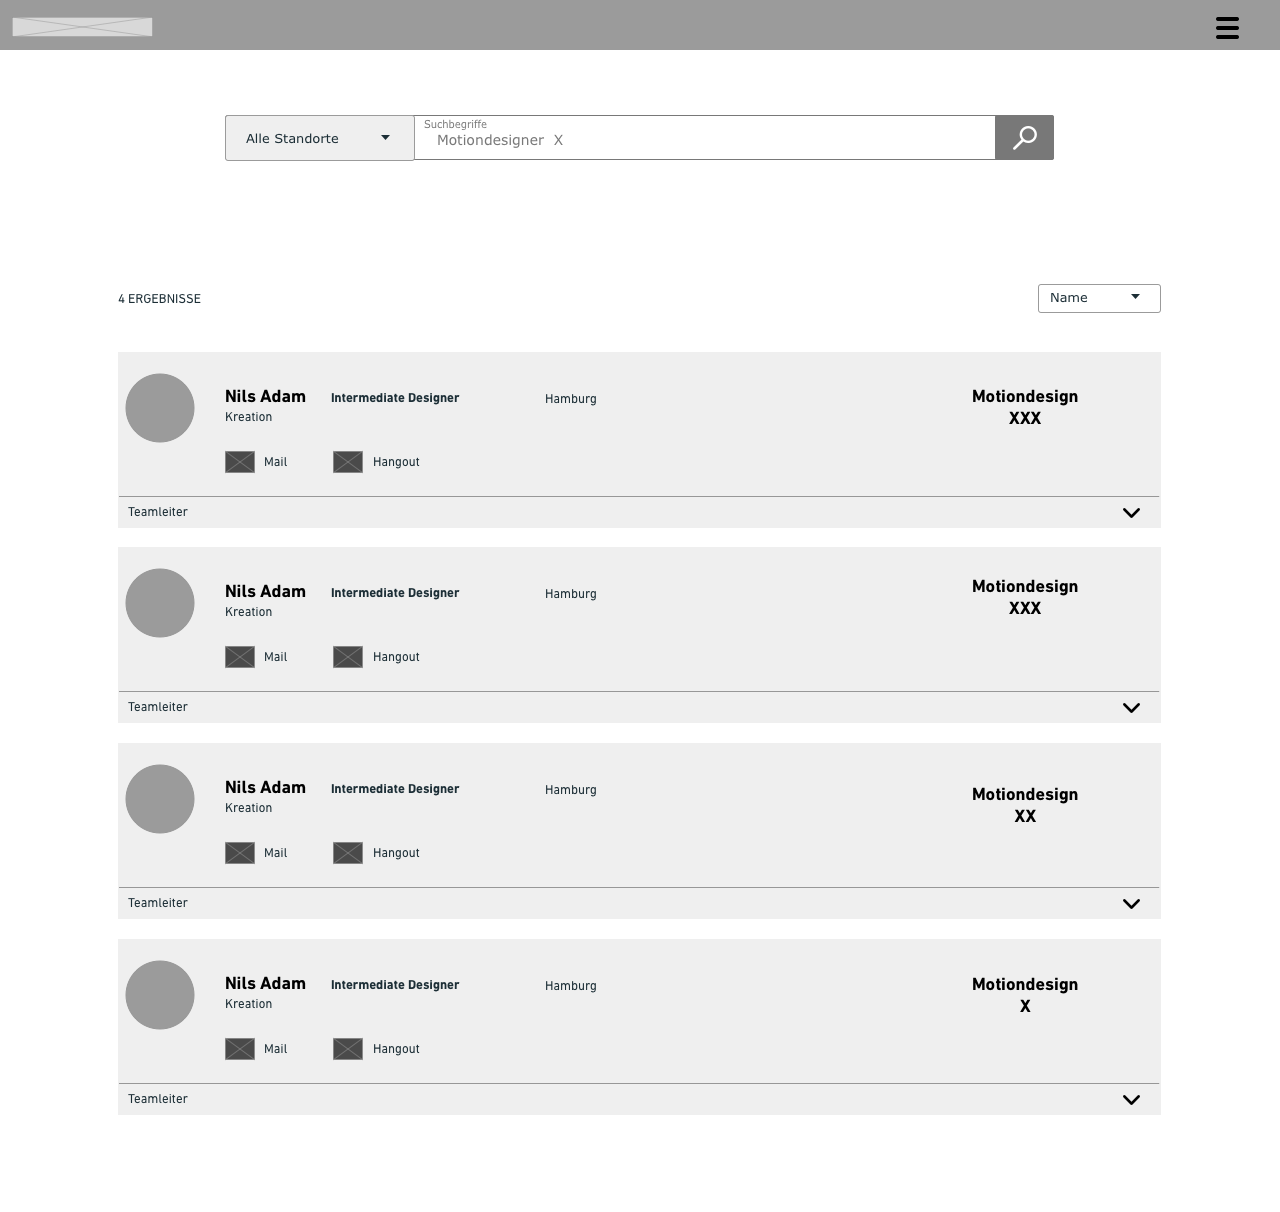
\includegraphics[width=\textwidth]{images/wireframe.png}
    \caption[Illustration: Search Result Page (Wireframe)]{Wireframe of the search result view}
    \label{fig:wireframe}
\end{figure}

\begin{figure}[p]
    \centering
    
\includegraphics[width=\textwidth]{images/design_home.png}
    \caption[Illustration: Search Page (Concept)]{An early prototypical design for the search view}
    \label{fig:design_home}
\end{figure}

\newpage

\section{Legal Concerns}
\label{legal_concerns}
The information saved in the system fall into the category of personal data (\textit{Personenbezogene Daten}), which is defined as ``any information concerning the personal or material circumstances of an identified or identifiable individual (the data subject)'' (BDSG, 3(1)). The personal data will be collected (BDSG, 3(3)), processed (BDSG, 3(4)) and transferred (BDSG, 3(3)) to other employees of SinnerSchrader.
Generally, this does not violate any law, since the ``collection, storage, modification or transfer of personal data or their use as a means of fulfilling one’s own business purposes shall be admissible'' (BDSG, 28(1)) but some restrictions apply: the data subjects have to be informed about the processing of their personal data, they must be able to deny their consent (BDSG, 4a), and the personal data shall not be made public.
To ensure the latter, the application must not be accessible to persons that do not work for or on behalf of SinnerSchrader. Technically, this will be arranged by making the application attainable from SinnerSchrader's internal network only which can exclusively be accessed by employees and authorized persons.\\
Furthermore, the Works Constitution Act (\textit{Betriebsverfassungsgesetz}) defines the rights and roles of the works council (\textit{Betriebsrat}) which have an impact on the design of the application. It states that ``the works council shall have a right of co-determination in the introduction and use of technical devices designed to monitor the behaviour or performance of the employees'' (BetrVG, 87(6)); since the application describes the employees' knowledge which is a key factor to their performance, this definition applies to it, so that the works council had to be involved in the design process.
Regarding the possibility for users to rate each other's skills as described in \ref{peerrating}, the council exercised its rights to object and interdicts its implementation because of both legal reasons and the personal concerns of employees; the council's statement can be found in appendix \ref{statement_br}.
